\section{Results}

The results include the time-dependent resources required 
for each of the scenarios described. This includes 
the number of reactors, mass of enriched uranium, and the 
\gls{SWU} capacity needed to produce the enriched uranium.
Results presented here are for fuel cycle scenarios 1-3.  

Figure \ref{fig:rx_deployment} shows the total number 
of each type of reactor deployed in each of the simulated 
scenarios. All scenarios deploy the same number of \gls{LWR}s. 
Each of the transitions utilize a \Cycamore \texttt{GrowthRegion} 
to control the deployment of the advanced reactor as needed 
to meet the specified demand, while the \gls{LWR}s are 
deployed at their specified start date. All of the scenarios 
have the same deployment schedule for \gls{LWR}s. To meet the
specified power demand of the transition, 5962 
\gls{MMR} reactors and 795 Xe-100 reactors are required.  


\begin{figure}[ht]
    \centering
    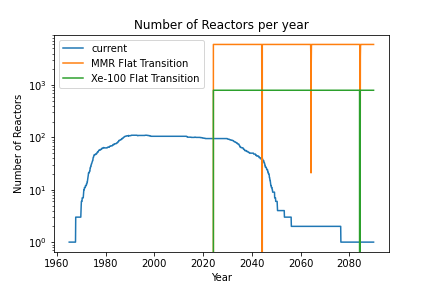
\includegraphics[scale=0.5]{figures/rx_deployment_all.png}
    \caption{Deployment of each type of reactor. \gls{LWR}s follow 
    the same deployment schedule in each scenario.}
    \label{fig:rx_deployment}
\end{figure}

Figure \ref{fig:energy} shows the total energy output from 
all of the reactors in each scenario. Each of the scenarios
have very similar energy outputs from the \gls{LWR}s, then 
show large differences in the energy output of the advanced 
reactors. The energy output in 
each of the transition scenarios does not match the flat demand 
starting at 2025 specified by the \Cycamore \texttt{GrowthRegion}. 
This is due to 
the use of mutual transactions in the \gls{DRE} 
\cite{gidden_methodology_2016}, which requires that each 
material request filled must be filled in full. Thus, we had to be 
cap the inventory of feed material (UF$_6$ commodity) that 
the enrichment facility could store. Placement of this cap to ensure 
use of both material streams causes small discrepancies in the 
energy output of the \gls{LWR}s. Further work is required 
to determine the cap on feed material inventory to better meet 
the intended energy demand of the transitions. Scenario 3 more 
closely matches the energy demand than scenario 2, likely because of the 
longer lifetime of the Xe-100 reactor. Scenario 2 never reaches 
the required power level. 

\begin{figure}[ht]
    \centering
    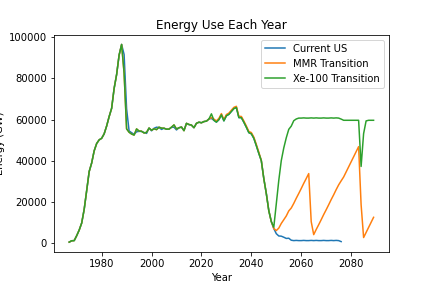
\includegraphics[scale=0.5]{figures/energy_all.png}
    \caption{Total energy output from reactors in each scenario.}
    \label{fig:energy}
\end{figure}

Figure \ref{fig:enriched_u} shows the amount of \gls{HALEU} 
required by scenarios 2 and 3. 
Both scenarios show a spike in \gls{HALEU} demand in 1975, which is
an artifact of the \gls{DRE} and is not due to the reactors' fuel 
requirements. Looking at the demand of \gls{HALEU} after 2049, scenario 2
requires 4556-6409 kg more than scenario 3, except for a single 
time step in 2084 when 
scenario 3 requires almost 69,000 kg more. This 
sudden spike in enriched uranium demand is due to the 
deployment of more Xe-100 reactors after the initial set 
of reactors reach their lifetime. 

\begin{figure}[ht]
    \centering
    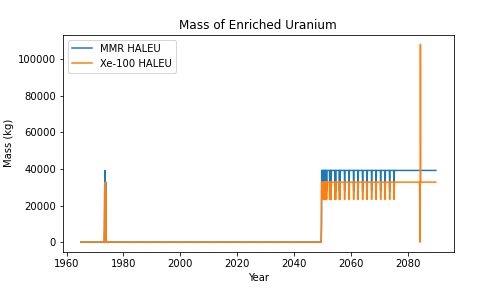
\includegraphics[scale=0.5]{figures/enrichedU_advancedrx.png}
    \caption{Enriched uranium demand for reactors.}
    \label{fig:enriched_u}
\end{figure}

Finally, Figure \ref{fig:swu} shows the \gls{SWU} required to 
produce enriched uranium in each scenario. The calculated 
\gls{SWU} for scenrios 2 and 3 includes \gls{SWU} to 
produce \gls{HALEU} for the advanced reactor and the \gls{LEU}
to produce fuel for the \gls{LWR}s. \gls{SWU} requirements 
clearly increase from scenario 1 to the 
transition scenarios once the advanced reactors are fueled. 
For most of the time steps in which the advanced reactors 
require fuel, scenario 3 requires 22,881 kg-SWU 
more than scenario 2, despite scenario 2 requiring a larger 
mass of \gls{HALEU}. This is because the Xe-100 reactors 
in scenario 3 require a higher level of enrichment.  

\begin{figure}[ht]
    \centering
    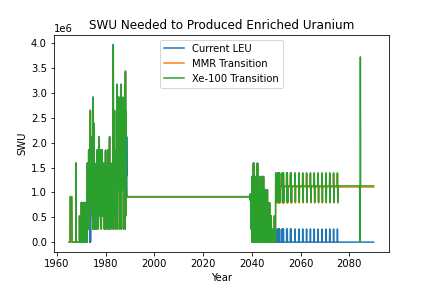
\includegraphics[scale=0.5]{figures/swu_all.png}
    \caption{Enriched uranium demand for reactors.}
    \label{fig:swu}
\end{figure}